\documentclass[handout]{beamer}

\usepackage{pgfpages}
%\pgfpagesuselayout{2 on 1}[a4paper,border shrink=5mm]
\usepackage{amsmath,amssymb,amsthm,array}
\usepackage{bm}
\usepackage{multirow}
\usepackage{multicol}
\usepackage{algorithm}
\usepackage{hyperref}
\usepackage{algorithmic}
\usepackage[normalem]{ulem}
\usepackage{fontspec}

\hypersetup{
    colorlinks=false,      		 % false: boxed links; true: colored links
    citecolor=red,       		 % color of links to bibliography
   	urlcolor=blue,          	 % color of external links 
  	linkbordercolor=red,	     % hyperlink borders will be red
 	pdfborderstyle={/S/U/W 1}	% border style will be underline of width 1pt
}

\usetheme{metropolis}

\title{Μοντέλα και Αποδείξεις Ασφάλειας στην Κρυπτογραφία - Ανταλλαγή Κλειδιού Diffie Hellman}
\author{Παναγιώτης Γροντάς - Άρης Παγουρτζής}
\date{30/10/2018}
\defbeamertemplate*{footline}{shadow theme}
{%
  \leavevmode%
  \hbox{
		\begin{beamercolorbox}[wd=.4\paperwidth,ht=2.5ex,dp=1.125ex,leftskip=.3cm,rightskip=.3cm plus1fil]{title in head/foot}%
			\usebeamerfont{title in head/foot} Formal Models - DHKE  %
		\end{beamercolorbox}
		\begin{beamercolorbox}[wd=.5\paperwidth,ht=2.5ex,dp=1.125ex,leftskip=.3cm,rightskip=.3cm plus1fil]{title in head/foot}%
			\usebeamerfont{title in head/foot} \hfill \insertsection  %
		\end{beamercolorbox}
		\begin{beamercolorbox}[wd=.1\paperwidth,ht=2.5ex,dp=1.125ex,leftskip=.3cm plus1fil,rightskip=.3cm]{author in head/foot}%
			\usebeamerfont{author in head/foot}\insertframenumber\,/\,\inserttotalframenumber
		\end{beamercolorbox}%
  }%
  \vskip0pt%
}
\institute{ΕΜΠ - Κρυπτογραφία (2018-2019)}

\setlength{\columnseprule}{0.38pt}
\begin{document}

\newcommand{\MSG}{ \mathtt{M} }
\newcommand{\KEY}{ \mathtt{K} }
\newcommand{\CPH}{ \mathtt{C} }
\newcommand{\keygen}{\mathtt{KeyGen}}
\newcommand{\enc}{\mathtt{Encrypt}}
\newcommand{\dec}{\mathtt{Decrypt}}
\newcommand{\adv}{$\mathcal{A} \,$ }
\newcommand{\advb}{$\mathcal{B} \,$ }
\newcommand{\chal}{$\mathcal{C} \,$ }
\newcommand{\cs}{$\mathcal{CS} \,$ }
 

\newcommand{\twopartdef}[4]
{ 
		\begin{cases}
			#1 , #2 \\
			#3 , #4
		\end{cases} 
}
\begin{frame}
\titlepage
\end{frame}



\begin{frame}{Περιεχόμενα}
\begin{itemize}
\item Ορισμός Κρυπτοσυστήματος
\item Μοντελοποίηση αντίπαλου
\item Μοντελοποίηση ασφάλειας
\item Κρυπτογραφικές αποδείξεις
\item Εφαρμογή: Ανταλλαγή Κλειδιού Diffie Hellman
\end{itemize}
\end{frame}

\section{Ορισμοί}
\begin{frame}{Κρυπτοσύστημα}
\begin{itemize}
\item \cs$=(\MSG, \KEY, \CPH, \keygen, \enc, \dec)$ 
\item $\MSG$: Σύνολο Μηνυμάτων
\item $\KEY$: Σύνολο Κλειδιών
\item $\CPH$: Σύνολο Κρυπτοκειμένων \pause
\end{itemize}
\underline{Δημιουργία κλειδιού}
\begin{itemize}
\item $\keygen(1^\lambda) = (key_{enc},{key_{dec}}) \in \KEY^2$ 
\begin{itemize}
\item Πιθανοτικός Αλγόριθμος 
\item Το κλειδί συνήθως επιλέγεται \emph{ομοιόμορφα} από το $\KEY$ 
\item $\lambda:$ Παράμετρος ασφάλειας - πλήθος bits του κλειδιού \pause
\begin{itemize}
	\item Συμβολισμός στο μοναδιαίο ($\lambda$ '1'): Πολυπλοκότητα εκφράζεται ως προς το μέγεθος της εισόδου, όχι ως προς την αναπαράστασή της(λογαριθμική)
	\item Σημασία για χρόνο εκτέλεσης κρυπτογράφησης, προσπάθειας - πιθανότητα επιτυχίας 'σπασίματος'
\end{itemize}
\end{itemize}
\end{itemize}
\end{frame}

\begin{frame}{Κρυπτοσύστημα (2)}
\underline{Κρυπτογράφηση}

$\enc(key_{enc},m) = c \in \CPH$ 
\begin{itemize}
\item Ντετερμινιστικός Αλγόριθμος: Κάθε μήνυμα αντιστοιχεί σε ένα κρυπτοκείμενο
\item Πιθανοτικός Αλγόριθμος: Κάθε μήνυμα αντιστοιχεί σε ένα σύνολο πιθανών κρυπτοκειμένων \pause
\end{itemize}

\underline{Αποκρυπτογράφηση}

$\dec(key_{dec},c) = m$ \pause

\underline{Ορθότητα}

$\dec(key_{dec}, \enc(key_{enc}, m)) = m, \forall m \in \MSG$
\end{frame}

\begin{frame}{Παρατηρήσεις}
\begin{itemize}
\item Συμμετρικό Κρυπτοσύστημα $key_{enc} = key_{dec}$ \pause
\item Ασύμμετρο Κρυπτοσύστημα $key_{enc} \neq key_{dec}$ \pause
\begin{itemize}
\item Κρυπτογραφία Δημοσίου Κλειδιού 
\item Το $key_{enc}$ μπορεί να δημοσιοποιηθεί για την εύκολη ανταλλαγή μηνυμάτων 
\item Το $key_{dec}$ είναι μυστικό
\end{itemize}
\end{itemize}
\end{frame}

\begin{frame}{Ο αντίπαλος \adv}
\begin{itemize}
\item Στόχος: Να \emph{σπάσει} το κρυπτοσύστημα 
\item Δηλαδή, με δεδομένο το $c$:
\pause
\begin{itemize}
\item Να μάθει το κλειδί $k$; 
\pause
\begin{itemize}
\item Επίθεση Πυρηνικής Βόμβας
\item Θέλουμε να προστατεύσουμε το μήνυμα
\item Τετριμμένα $\enc(k,m)=m$ είναι αδύνατο να σπάσει, αλλά τι ασφάλεια παρέχει;
\end{itemize}
\pause
\item Να μάθει ολόκληρο το αρχικό μήνυμα $m$;
\begin{itemize}
\item Αν μάθει το 90\%;
\end{itemize}
\pause
\item Να μάθει κάποια συνάρτηση του $m$;
\begin{itemize}
\item Ναι αλλά ποια;
\end{itemize}
\end{itemize}
\pause
\item Συμπέρασμα:Χρειάζονται ακριβείς ορισμοί
\begin{itemize}
\item Για το τι σημαίνει 'σπάσιμο'
\item Για τις δυνατότητες και τα μέσα του αντιπάλου.
\end{itemize}
\end{itemize}
\end{frame}

\section{Είδη επιθέσεων}
 
\begin{frame}{Επίθεση Μόνο Κρυπτοκειμένου - Ciphertext Only Attack (COA)}
\begin{itemize}
\item Παθητικός Αντίπαλος (Eve)
\item Πολύ εύκολη: Χρειάζεται απλά πρόσβαση στο κανάλι επικοινωνίας
\end{itemize}
\end{frame}

\begin{frame}{Επίθεση Γνωστού Μηνύματος -  Known Plaintext Attack (KPA)}
\begin{itemize}
\item Παθητικός Αντίπαλος
\item Γνωρίζει \emph{ζεύγη μηνυμάτων - κρυπτοκειμένων}
\item Τετριμμένο σενάριο για ασύμμετρα, γιατί: \pause
\begin{itemize}
	\item O \adv έχει το δημόσιο κλειδί
	\item Μπορεί να κατασκευάσει μόνος του όσα ζεύγη θέλει
\end{itemize} \pause
\item Ρεαλιστικό σενάριο και για συμμετρικά, γιατί: \pause
\begin{itemize}
\item Ακόμα και τα κρυπτογραφημένα πρωτόκολλα περιέχουν μη απόρρητα μηνύματα (handshakes, ack)
\item Ιστορικό παράδειγμα: Κρυπτοκείμενα πρόγνωσης καιρού στη μηχανή Enigma
\item Κρυπτογραφημένα μηνύματα γίνονται κάποια στιγμή διαθέσιμα
\end{itemize} 
\end{itemize} 
\end{frame}

\begin{frame}{Επίθεση Επιλεγμένου Μηνύματος - Chosen Plaintext Attack (CPA)}
 
\begin{itemize}
\item \emph{Ενεργός} Αντίπαλος (Mallorie)
\item Γνωρίζει ζεύγη μηνυμάτων - κρυπτοκειμένων
\item \emph{Μπορεί να ζητήσει την κρυπτογράφηση μηνυμάτων της επιλογής του (Μαντείο Κρυπτογράφησης)} \pause
\item Ιστορικό Παράδειγμα: Σπάσιμο κρυπτοσυστήματος JN-25b στη ναυμαχία του Midway (Ιούνιος 1942)
\begin{itemize}
	\item Υποψία ότι $\enc(\text{"Midway"}) = \text{"AF"}$
	\item Αποστολή Πλαστών Μηνυμάτων για επισκευή του συστήματος υδροδότησης του 'Midway'
	\item Συλλογή Επικοινωνιών Με Κρυπτοκείμενα 'AF'
	\item Συσχέτιση με παλιότερες επικοινωνίες
\end{itemize}
\end{itemize}
\end{frame}



\begin{frame} {Επίθεση Επιλεγμένου Κρυπτοκειμένου - Chosen Ciphertext Attack (CCA)}
\begin{itemize}
\item Ενεργός Αντίπαλος
\item Γνωρίζει ζεύγη μηνυμάτων - κρυπτοκειμένων
\item Μπορεί να ζητήσει την κρυπτογράφηση μηνυμάτων της επιλογής του (Μαντείο Κρυπτογράφησης)
\item \emph{Μπορεί να επιτύχει την αποκρυπτογράφηση μηνυμάτων της επιλογής του (Μαντείο Αποκρυπτογράφησης)} \pause
\item Διαίσθηση: Ο αντίπαλος μπορεί να βγάλει \emph{έμμεσα} συμπεράσματα από αντιδράσεις σε κρυπτογραφημένα μηνύματα
\begin{itemize}
\item Απόρριψη κρυπτογραφημένων 'σκουπιδιών' από το πρωτόκολλο (Bleichenbacher RSA PKCS1 attack)
\item Ενέργεια στον πραγματικό κόσμο (πχ. αγορά μετοχών)
\item Ιστορικό (αντιπαράδειγμα:) Μη αποτροπή του βομβαρδισμού του Coventry
\end{itemize}
\end{itemize}
\end{frame}

\section{Μοντέλα Ασφάλειας}

\begin{frame}{Οι κανόνες του Kerchoffs (1883)}

Οι πρώτες προσπάθειες ορισμού ασφάλειας κρυπτοσυστημάτων και προστασίας 

\pause 

\begin{block}{Αρχή 2}
Ο αλγόριθμος(από)κρυπτογράφησης δεν πρέπει να είναι μυστικός. Πρέπει να μπορεί να πέσει στα χέρια του \adv χωρίς να δημιουργήσει κανένα πρόβλημα. Αντίθετα το κλειδί μόνο πρέπει να είναι μυστικό.
\end{block}

Λόγοι: \pause 

\begin{itemize}
\item Tο κλειδί διανέμεται πιο εύκολα από τους αλγόριθμους (μικρότερο μέγεθος, απλούστερη δομή)  
\item Το κλειδί είναι πιο εύκολο να αλλαχθεί αν διαρρεύσει
\item Πιο πρακτική χρήση για περισσότερους από έναν συμμετέχοντες
\item Ανοικτό κρυπτοσύστημα: Εύκολη μελέτη 
\end{itemize}

\end{frame}

\begin{frame}{Οι κανόνες του Kerchoffs (1883) - (2)}
Παρατηρήσεις:

Αν και έχουν παράδοση ακόμα και σήμερα δεν εφαρμόζονται πλήρως
\begin{itemize}
\item (Μεγάλες) εταιρίες δημιουργούν και χρησιμοποιούν δικούς τους μυστικούς αλγόριθμους/πρωτόκολλα \pause

\item Bruce Schneier \href{https://goo.gl/FaFoSK}{Crypto Snake Oil}
\end{itemize}

\end{frame}
 

\begin{frame}{Οι κανόνες του Kerchoffs (1883) - (3)}
\begin{block}{Αρχή 1}
Το κρυπτοσύστημα θα πρέπει να είναι \emph{πρακτικά} απρόσβλητο, αν δεν γίνεται θεωρητικά
\end{block}

\begin{itemize}
\item Διάρκεια Κρυπτανάλυσης > Διάρκεια Ζωής Μηνύματος
\item Μικρή Πιθανότητα Επιτυχίας
\item Υπολογιστική Ασφάλεια
\end{itemize}
\pause 

Εμπειρική αρχή - δεν αντιστοιχίζονται σε κάτι πρακτικό
\end{frame}

\begin{frame}{Αποδείξιμη Ασφάλεια}

\begin{block}{Ιδέα}
Μαθηματική (Λογική) απόδειξη ότι το κρυπτοσύστημα έχει κάποιες ιδιότητες ασφάλειας.
\end{block}

Παράδειγμα: Τέλεια μυστικότητα (Shannon) \pause

Μπορεί να εφαρμοστεί στην κρυπτογραφία δημοσίου κλειδιού; Γιατί;

\pause 

Επαναχρησιμοποίηση δημοσίου κλειδιού

\end{frame}

\begin{frame}{Σημασιολογική Ασφάλεια}
Βασική ιδέα (Goldwasser, Micali): 

Χαλαρώνουμε τις απαιτήσεις ασφάλειας για να οδηγηθούμε σε έναν πιο χρήσιμο ορισμό

\pause
Λαμβάνουμε υπ'όψιν:

\begin{itemize}
	\item την υπολογιστική ισχύ του \adv
	\item την πιθανότητα επιτυχίας
	\item το είδος των επιθέσεων
\end{itemize}

\pause
\begin{block}{Διαίσθηση}
Ένας υπολογιστικά περιορισμένος \adv  δεν μπορεί να μάθει τίποτε χρήσιμο από το κρυπτοκείμενο παρά μόνο με αμελητέα πιθανότητα
\end{block}
\end{frame}

\begin{frame}{Ρητή Προσέγγιση}

\begin{block}{Ορισμός}
Ένα κρυπτοσύστημα είναι $(\tau,\epsilon)$ ασφαλές αν οποιοσδήποτε \adv σε χρόνο το πολύ $\tau$, δεν μπορεί να το σπάσει με πιθανότητα καλύτερη από $\epsilon$ 
\end{block}

\pause

Παράδειγμα: Για συμμετρικά κρυπτοσυστήματα σήμερα με μακροχρόνια απαιτήσεις ασφάλειας $2^{80} < \tau < 2^{100}$ και $\epsilon=2^{-64}$
Στατιστικά distributed.net brute force cracking:
\begin{itemize}
	\item 56bits - 250 μέρες 
	\item Παγκόσμιο ρεκόρ: 2002 - 64bits -  5 χρόνια
	\item Τώρα: Προσπάθεια για σπάσιμο κλειδιού 72bits (μετά 15 χρόνια έχει εξερευνηθεί το 5\% του $\KEY$)
	\item Quantum computers: $2^{\tau/2}$ generic speedup (αλγόριθμος Grover)
\end{itemize}
\end{frame}

\begin{frame}{Ρητή Προσέγγιση (2)}
\alert{Δεν χρησιμοποιείται} γιατί: \pause

\begin{itemize}
\item Δεν ασχολείται με το υπολογιστικό μοντέλο (κατανεμημένοι υπολογιστές, εξειδικευμένο HW κτλ.)
\item Δεν ασχολείται με το τι θα γίνει μετά το $\tau$
\item Για τους ίδιους λόγους με Υπολογιστική Πολυπλοκότητα
\end{itemize}
\end{frame}

\begin{frame}{Ασυμπτωτική Προσέγγιση}
\begin{block}{Ορισμός}
Ένα κρυπτοσύστημα είναι ασφαλές αν οποιοσδήποτε περιορισμένος \adv έχει αμελητέα πιθανότητα να το σπάσει (σε σχέση με την παράμετρο ασφάλειας)
\end{block}
\pause
Παρατηρήσεις:
\begin{itemize}
	\item περιορισμένος = Probabilistic Polynomial Time
	\item Ισχύει για μεγάλες τιμές του $\lambda$
	\item Συνέπεια του $|\KEY| < |\MSG|$
	\item Επιτρέπει προσαρμογή της ασφάλειας με αλλαγή του μήκους του κλειδιού
\end{itemize}
\end{frame}

\begin{frame}{Στόχος αντιπάλου}

\begin{itemize}
\item O \adv θέλει να υπολογίσει το κατηγόρημα $q: \MSG \rightarrow \{0,1\}$ \pause
\item Γενικά: $Pr_{m \in \MSG}[q(m)=0]=Pr_{m \in \MSG}[q(m)=1]=\frac{1}{2}$
\item Το μήκος των κρυπτοκειμένων είναι το ίδιο (δεν διαρρέει πληροφορία)
\end{itemize}

\pause

\begin{block}{Το πλεονέκτημα του \adv}
$Adv_q(\mathcal{A}) = |Pr[\mathcal{A}(c)=q(\dec(key,c))]-\frac{1}{2}|$
\end{block}
\pause

Αν ο \adv μαντέψει στην τύχη έχει $Adv_q(\mathcal{A})=0$

\end{frame}


\begin{frame}{Σημασιολογική ασφάλεια - ορισμός}
\begin{block}{Ορισμός}
Ένα κρυπτοσύστημα είναι σημασιολογικά ασφαλές όταν $\forall$ PPT \adv, $\forall q$:
\begin{center}
$Adv_q(\mathcal{A})=negl(\lambda)$
\end{center}
\end{block}

\pause

\begin{block}{Αμελητέα συνάρτηση}
Οποιαδήποτε συνάρτηση για την οποία για κάθε πολυώνυμο $p$ υπάρχει $n_0$ ώστε $\forall n \geq n_0: neql(n)<\frac{1}{p(n)}$
\end{block}

Δηλαδή: Μεγαλώνει με πιο αργό ρυθμό από αντίστροφο πολυώνυμο

Για παράδειγμα: $2^{-n},2^{-\sqrt{n}},n^{-log{n}} $
 
\end{frame}

\begin{frame}{Σημασιολογική ασφάλεια (2)}
\begin{block}{Παρατηρήσεις}
\begin{itemize}
\item Ο τυπικός ορισμός ενσωματώνει την παράμετρο ασφαλείας
\item Δύσχρηστος ορισμός - δεν ορίζουμε τι ξέρει ο \adv και τι διαδικασία  ακολουθεί για το 'σπάσιμο'
\end{itemize}
\end{block}
\end{frame}

\begin{frame}{Μη Διακρισιμότητα (Indistinguishability)}

Οντότητα  (challenger - αναπαριστά το κρυπτοσύστημα)

Παίγνιο Μη Διακρισιμότητας μεταξύ των \adv, \chal

\begin{figure} 
	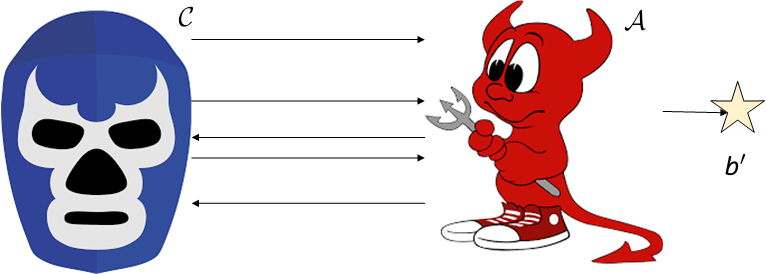
\includegraphics[scale=0.3]{game.png}  
\end{figure}
 
\begin{itemize}
	\item Ανταλλαγή Μηνυμάτων μεταξύ \adv, \chal \pause
	\item \adv: Παράγει δύο μηνύματα $m_0, m_1$ \pause
	\item \chal: Διαλέγει ένα τυχαίο bit $b$ \pause
	\item \chal: Παράγει και απαντά με το $c_b = \enc(m_b)$ \pause
	\item \adv: Μαντεύει ένα bit $b'$ \pause
	\item Κερδίζει αν μαντέψει την επιλογή του αντιπάλου
\end{itemize}	
 
\end{frame}

\begin{frame}{Μη Διακρισιμότητα (Indistinguishability) - (2)}

\begin{block}{Δηλαδή:}
$IND-Game(\mathcal{A}) = \twopartdef{1}{b'=b}{0}{\text{αλλιώς}}$
\end{block}

\begin{block}{Πλεονέκτημα}
$Adv_{IND}(\mathcal{A}) = |Pr[IND-Game(\mathcal{A})=1]-\frac{1}{2}|$
\end{block}
\pause
\begin{block}{Ορισμός}
Ένα κρυπτοσύστημα  διαθέτει την ιδιότητα της μη διακρισιμότητας όταν $\forall$ PPT \adv:
\begin{center}
$Adv_{IND}(\mathcal{A}) = negl(\lambda)$
\end{center}
\end{block}
\pause
\begin{block}{Θεώρημα}
Σημασιολογική Ασφάλεια $\Leftrightarrow$ Μη-Διακρισιμότητα
\end{block}
\end{frame}

\begin{frame}{IND-EAV}
\begin{figure} 
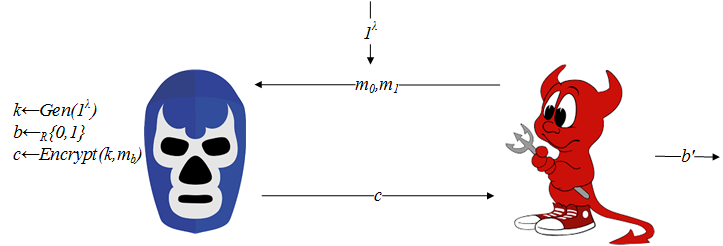
\includegraphics[scale=0.6]{ind-eav.png}  
\end{figure}
\end{frame}

\begin{frame}{IND-CPA}
\begin{figure} 
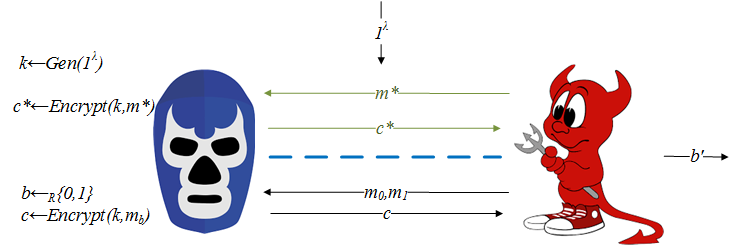
\includegraphics[scale=0.6]{ind-cpa.png}  
\end{figure}
\end{frame}

\begin{frame}{Παρατηρήσεις IND-CPA}
\begin{block}{Θεώρημα}
Ένα κρυπτοσύστημα με ντετερμινιστικό αλγόριθμο κρυπτογράφησης δεν μπορεί να έχει την ιδιότητα IND-CPA.
\end{block}
{Απόδειξη}
\pause

\begin{itemize}
\item O \adv θέτει $m^*=m_0$ και λαμβάνει την κρυπτογράφηση $c^*$
\item Η απάντηση του είναι $b'=\twopartdef{0}{c^*=c}{1}{\text{αλλιώς}}$
\item O \adv κερδίζει πάντα $Pr[IND-CPA(\mathcal{A})=1]=1$
\end{itemize}

\end{frame}
\begin{frame}{IND-CCA}
\begin{figure} 
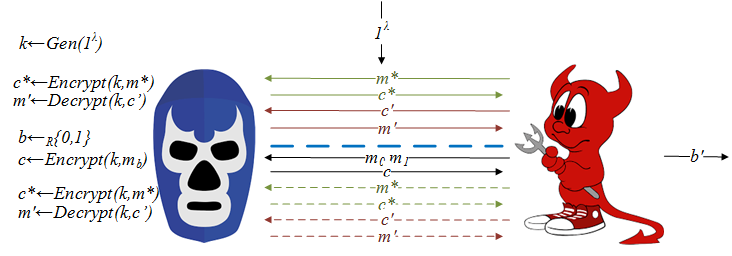
\includegraphics[scale=0.6]{ind-cca.png}  
\end{figure}
\end{frame}

\begin{frame}{Παρατηρήσεις}
\begin{itemize}
\item Παραλλαγή IND-CCA2: Επιτρέπεται χρήση του μαντείου αποκρυπτογράφησης μετά το $c$ (adaptive IND-CCA)
\item Παραλλαγή IND-CCA1: αλλιώς \pause
\item Στο παίγνιο IND-CCA o \adv δεν μπορεί να ρωτήσει τον $C$ για την αποκρυπτογραφήση του $c$ \pause
\item Μπορεί όμως να:
\begin{itemize}
\item Μετατρέψει το $c$ σε $\hat{c}$
\item Ζητήσει την αποκρυπτογράφηση του $\hat{c}$ σε $\hat{m}$
\item Να μετατρέψει το $\hat{m}$ σε $m$, κερδίζοντας με πιθανότητα 1
\end{itemize} 

\end{itemize}
\end{frame}

\begin{frame}{Malleability}

Χειρισμός κρυπτοκειμένων χωρίς αποκρυπτογράφηση

\begin{block}{\emph{Malleable (εύπλαστο)} Κρυπτοσύστημα}
Επιτρέπει στον \adv να φτιάξει, γνωρίζοντας μόνο το κρυπτοκείμενο $c=\enc(m)$, ένα \emph{έγκυρο} κρυπτοκείμενο $c'=\enc(h(m))$, για κάποια, συνήθως πολυωνυμικά αντιστρέψιμη, συνάρτηση $h$ γνωστή σε αυτόν. 
\end{block}

\pause
Κάποιες φορές είναι επιθυμητή και κάποιες όχι.
\begin{itemize}
\item Ομομορφικά Κρυπτοσυστήματα: Αποτίμηση μερικών πράξεων στα κρυπτοκείμενα (ηλ. ψηφοφορίες) \pause
\item Πλήρως Ομομορφικά Κρυπτοσυστήματα (Gentry 2010): Αποτίμηση οποιουδήποτε κυκλώματος στα κρυπτοκείμενα \pause
\item Δεν μπορούν να είναι IND-CCA2, ... αλλά είναι πολύ χρήσιμα \pause
\end{itemize}
\pause
\begin{block}{Σημαντική ιδιότητα}
Non-malleability $\Leftrightarrow$ IND-CCA2
\end{block}
\end{frame}

\section{Αποδείξεις Ασφάλειας}

\begin{frame}{Κρυπτογραφικές Αναγωγές}
\begin{block}{Γενική Μορφή}
Αν ισχύει η υπόθεση $\mathcal{Y}$, τότε και το κρυπτοσύστημα \cs είναι ασφαλές (υπό συγκεκριμένο ορισμό).
\end{block}
\pause

\begin{block}{Αντιθετοαντιστροφή}
Αν το \cs ΔΕΝ είναι ασφαλές (υπό συγκεκριμένο ορισμό), τότε δεν ισχύει η $\mathcal{Y}$.
\end{block}
\end{frame}

\begin{frame}{Κατασκευαστική απόδειξη}
 
\begin{itemize}
\item \cs μη ασφαλές $\Rightarrow$ $\exists$ PPT \adv  o οποίος παραβιάζει τον ορισμό ασφάλειας
\item \emph{Κατασκευάζουμε} PPT αλγόριθμο  $\mathcal{B}$, ο οποίος αλληλεπιδρά με τον $\mathcal{C}_y$ ο οποίος προσπαθεί να 'υπερασπιστεί' την $\mathcal{Y}$
\item Ο $\mathcal{B}$ για να καταρρίψει την $\mathcal{Y}$ χρησιμοποιεί εσωτερικά σαν υπορουτίνα τον \adv (black box access) παριστάνωντας τον $\mathcal{C}$ στο παίγνιο μη διακρισιμότητας του \cs
\end{itemize}
\end{frame}

\begin{frame}{Σχηματικά}
\begin{figure}
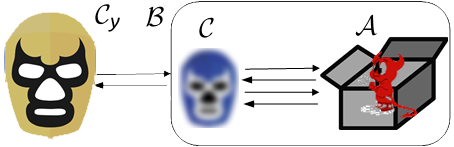
\includegraphics[scale=0.8]{ProofReduction.png}  
\end{figure}
\end{frame}

\begin{frame}{Παρατηρήσεις}
Κανόνες Ορθότητας
\begin{itemize}
	\item Προσομοίωση: Ο \adv δεν θα πρέπει να ξεχωρίζει τον $\mathcal{B}$ από οποιονδήποτε άλλο εισηγητή.
	\item Πιθανότητα επιτυχίας: Αν ο \adv έχει μη αμελητέα πιθανότητα επιτυχίας τότε και ο $\mathcal{B}$ θα πρέπει να έχει μη αμελητέα πιθανότητα
	\item Πολυπλοκότητα: Ο $\mathcal{B}$ θα πρέπει να είναι PPT. Αυτό πρακτικά σημαίνει ότι όποια επιπλέον εσωτερική επεξεργασία  πρέπει να είναι πολυωνυμική  
	\item Πρέπει να είναι όσο πιο tight γίνεται ($t_\mathcal{B} \approx t_\mathcal{A}$ και $\epsilon_\mathcal{B} \approx \epsilon_\mathcal{A}$)
\end{itemize}
\end{frame}

\begin{frame}{Συμπεράσματα-Συζήτηση}
Κρυπτογραφικές Αναγωγές
\begin{itemize}
\item Παρέχουν σχετικές εγγυήσεις (Δύσκολο Πρόβλημα, Μοντέλο Ασφάλειας) \pause
\item Δίνουν ευκαιρία να ορίσουμε καλύτερα το κρυπτοσύστημα/πρωτόκολλο \pause
\item Πρακτική Χρησιμότητα: Ρύθμιση Παραμέτρου Ασφάλειας \pause
\item Συγκέντρωση Κρυπταναλυτικών Προσπαθειών στο Πρόβλημα Αναγωγής και όχι σε κάθε κρυπτοσύστημα ξεχωριστά \pause
\item Πιο σημαντικές όσο πιο πολύπλοκο γίνεται το πρωτόκολλο \pause
\item Αποδεικνύουν την ασφάλεια του μοντέλου, αλλά: 
\begin{itemize}
	\item Πόσο αναπαριστά το μοντέλο την πραγματικότητα; #KRACK \pause
	\item Δεν σημαίνει ότι οποιαδήποτε υλοποίηση θα είναι ασφαλής
\end{itemize}
\end{itemize}

\end{frame}\section{Ανταλλαγή Κλειδιού Diffie Hellman}
\begin{frame}{Το πρωτόκολλο DHKE}
Αντί για Alice και Bob... \pause
\begin{center}
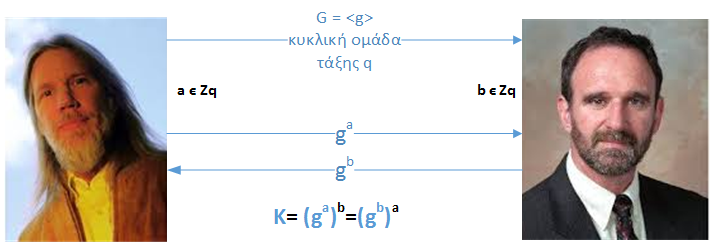
\includegraphics[scale=0.45]{dh.png}
\end{center} 
\pause
Πρωτόκολλο \textbf{Δημιουργίας} Κλειδιού \\
\pause
\textbf{Απαιτήσεις}: \\
Ασφάλεια: Ύψωση σε δύναμη - μονόδρομη συνάρτηση στην $\mathbb{G}$
\pause 
Συνήθως: $\mathbb{G}$ υποομάδα του $\mathbb{Z}_p^*$ με $p$ πρώτο ή ελλειπτικές καμπύλες\\
\pause
Εφαρμογές: SSL, TLS, IPSEC
\end{frame}

\begin{frame}{Ασφάλεια DHKE - Πρόβλημα DLP}

\begin{block}{DLP - Το πρόβλημα του Διακριτού Λογάριθμου}
Δίνεται μια κυκλική ομάδα $\mathbb{G}=\langle g \rangle$ τάξης $q$ και ένα τυχαίο στοιχείο $y \in \mathbb{G}$

Να υπολογιστεί $x \in \mathbb{Z}_q$ ώστε $g^x = y$ \\
δηλ. το $log_g y \in \mathbb{Z}_q$
\end{block}
\pause
\alert{Αγνοούμε δεδομένα στο πρωτόκολλο DHKE}
\end{frame}

\begin{frame}{Ασφάλεια DHKE - Πρόβλημα CDHP}
\begin{block}{CDHP - Το υπολογιστικό πρόβλημα Diffie Hellman}
Δίνεται μια κυκλική ομάδα $\mathbb{G}=\langle g \rangle$, δύο στοιχεία $y_1=g^{x_1}, y_2 = g^{x_2}$

Να υπολογιστεί το $g^{x_1 \cdot x_2}$ 
\end{block}
\end{frame}

\begin{frame}{Ασφάλεια DHKE - Πρόβλημα DDHP}
\green{Μπορούμε να δοκιμάζουμε τυχαία στοιχεία}

\begin{block}{DDHP - Το πρόβλημα απόφασης Diffie Hellman}
Δίνεται μια κυκλική  ομάδα $\mathbb{G}=\langle g \rangle$, δύο στοιχεία $y_1=g^{x_1}, y_2 = g^{x_2}$ και κάποιο  $y \in \mathbb{G}$ 

Να εξεταστεί αν  $y = g^{x_1 \cdot x_2}$ 
\end{block}
\pause
ή ισοδύναμα
\begin{block}{DDHP - Το πρόβλημα απόφασης Diffie Hellman}
Δίνεται μια κυκλική  ομάδα $\mathbb{G}=\langle g \rangle$, δύο στοιχεία $y_1=g^{x_1}, y_2 = g^{x_2}$ και κάποιο  $y \in \mathbb{G}$ 

Μπορούμε να ξεχωρίσουμε τις τριάδες ($g^{x_1}, g^{x_2}, g^{x_1 x_2}$) και  ($g^{x_1}, g^{x_2}, y$);
\end{block}
\end{frame}

\begin{frame}{DDH σε μορφή παιγνίου $DDH-Game$}
\begin{small}
Κοινή είσοδος: παράμετρος ασφάλειας $\lambda$.

Λειτουργίες \chal
\begin{itemize}
	\item Παραγωγή: $\mathbb{G}=\langle g \rangle$ τάξης πρώτου $q$. 
	\item Επιλογή τυχαίων $x_1,x_2 \in \mathbb{Z}_q$, $y \in G$
	\item Υπολογισμός $g^{x_1}, g^{x_2}, g^{x_1 x_2}$
	\item Επιλογή τυχαίου bit $b \in \{ 0,1 \}$
	\item Αν $b=0$ τότε αποστολή $\mathbb{G}, g^{x_1}, g^{x_2}, y' = g^{x_1 x_2}$ στον \adv
	\item Αν $b=1$ τότε αποστολή $\mathbb{G}, g^{x_1}, g^{x_2},y' = y$ στον \adv
\end{itemize}	

O \adv υπολογίζει $b'$. 

Αν $b'\neq b$ τότε το αποτέλεσμα του παιχνιδιού είναι $0$, αλλιώς $1$
\end{small}
\end{frame}

\begin{frame}{DDH σε μορφή παιγνίου $DDH-Game$ (2)}

Πλεονέκτημα \adv:

\begin{align*} Adv_{\mathcal{A}}^{DDH-Game} = \\
| Pr[DDH-Game(\mathcal{A}(\mathbb{G},g^{x_1}, g^{x_2}, g^{x_1 x_2})=1)] \\
  - Pr[DDH-Game(\mathcal{A}(\mathbb{G},g^{x_1}, g^{x_2}, y)=1)] |
\end{align*}

Η υπόθεση DDH ισχύει αν $\forall$ PPT:

$\mathcal{A}$: $Adv_{\mathcal{A}}^{DDH}(\lambda) = negl(\lambda)$

\end{frame}

\begin{frame}{Σχέσεις Προβλημάτων}
\begin{block}{$CDHP \leq DLP$}
Αν μπορούμε να λύσουμε το $DLP$, τότε μπορούμε να υπολογίζουμε τα $x_1, x_2$ από τα $y_1, y_2$ και στην συνέχεια το $g^{x_1 \cdot x_2}$
\end{block}

\pause
 
\begin{block}{$DDHP \leq CDHP$}
Αν μπορούμε να λύσουμε το $CDHP$, υπολογίζουμε το $g^{x_1 \cdot x_2}$ και ελέγχουμε ισότητα με το $y$
\end{block}
 
\pause 
Δηλαδή: $DDHP \leq CDHP \leq DLP$

\alert{Δεν γνωρίζουμε αν ισχύει η αντίστροφη σειρά - ισοδυναμία}
\alert{Όμως:}
Υπάρχουν ομάδες όπου το $DDHP$ έχει αποδειχθεί εύκολο, ενώ $CDHP$ δεν έχει αποδειχθεί εύκολο\\
\alert{Μάλλον:} $DDHP < CDHP$
\end{frame}

\begin{frame}{Ασφάλεια DHKE}
Μοντέλο ασφάλειας: παθητικός αντίπαλος \adv
\begin{block}{Διαίσθηση}
O \adv  δεν αποκτά καμία χρήσιμη πληροφορία για το κλειδί που δημιουργείται.\\
\green{Ισοδύναμα}\\
O \adv δεν μπορεί να διακρίνει το κλειδί από ένα τυχαίο στοιχείο της ομάδας στην οποία ανήκει
\end{block}
\end{frame}
 

\begin{frame}{Παιχνίδι ανταλλαγής κλειδιού $KEG(\lambda,\mathcal{A},\Pi)$}
Κοινή είσοδος: $\lambda$. Λειτουργίες \chal: 
\begin{itemize}
\item Δημιουργεί ομάδα $\mathbb{G}$
\item Εκτελεί το πρωτοκόλλο $\Pi(1^\lambda)$
\item Παράγεται: $(\tau,k)$
\begin{itemize}
	\item $\tau$: Τα μηνύματα που ανταλλάσσονται (δημόσια) 
	\item $k$: Το κλειδί που παράγεται (ιδιωτικό) 
\end{itemize}
\item Επιλογή τυχαίου $b \in \{0,1\}$ 
\item Αν $b = 0$ επιλογή τυχαίου $k'$ και αποστολή $(\tau,k')$ στον \adv
\item Αν $b = 1$ αποστολή $(\tau,k)$ στον \adv
\end{itemize}
O \adv υπολογίζει $b'$. Αν $b'\neq b$ τότε το αποτέλεσμα του παιχνιδιού είναι $0$, αλλιώς $1$

Πλεονέκτημα \adv:
$Adv_{\mathcal{A},\Pi}^{KEG}(\lambda) = | Pr[KEG_{\Pi}(\mathcal{A}(\tau,k)=1)]-Pr[KEG_{\Pi}(\mathcal{A}(\tau,k')=1)] |$

\end{frame}
 
\begin{frame}{Ορισμός ασφάλειας DHKE}
Ένα πρωτόκολλο ανταλλαγής κλειδιού $\Pi$ είναι ασφαλές, αν κάθε PPT \emph{παθητικός} αντίπαλος \adv έχει αμελητέα πιθανότητα ως προς την παράμετρο ασφάλειας να επιτύχει στο $KEG$
\green{$Prob[KEG(\lambda,\Pi,\mathcal{A})=1] \leq \frac{1}{2}+negl(\lambda)$}

\medskip

Ένα πρωτόκολλο ανταλλαγής κλειδιού $\Pi$ είναι ασφαλές, αν κάθε PPT \emph{παθητικός} αντίπαλος \adv έχει αμελητέo πλεονέκτημα ως προς την παράμετρο ασφάλειας να επιτύχει στο $KEG$
$Adv_{\mathcal{A},\Pi}^{KEG}(\lambda)(\lambda) = negl(\lambda)$
\end{frame}

\begin{frame}{Απόδειξη ασφάλειας DHKE}
\begin{small}
\alert{Αν το DDHP είναι δύσκολο, τότε το πρωτόκολλο DHKE είναι ασφαλές (απέναντι σε παθητικό αντίπαλο)}


\textbf{Απόδειξη - Σχεδιάγραμμα}
DHKE μη ασφαλές: $\exists$\adv ώστε \alert{$Adv_{\mathcal{A}}^{KEG}(\lambda) = non-negl(\lambda)$} 

Θα κατασκευάσουμε αντίπαλο PPT \advb ο οποίος παραβιάζει την $DDH$ με μη αμελητέο πλεονέκτημα. 

Ο \advb λειτουργεί ως εξής:
\begin{itemize}
	\item Όταν λάβει το μήνυμα από τον $\mathcal{C}_{DDH}$ το προωθεί στον \adv
	\item Μορφή μηνύματος $(\tau,k') = ((\mathbb{G}, g^{x_1}, g^{x_2})),y')$
	\item Όταν ο \adv απαντήσει, προωθεί το $b'$.
\end{itemize}

\begin{tiny}

\begin{align*}
Adv_{\mathcal{B}}^{DDH-Game} = | Pr[DDH-Game(\mathcal{B}(\mathbb{G},g^{x_1}, g^{x_2}, g^{x_1 x_2})=1)]-Pr[DDH-Game(\mathcal{B}(\mathbb{G},g^{x_1}, g^{x_2}, y)=1)] = \\
| Pr[KEG_{DHKE}(\mathcal{A}(\tau,k)=1)]-Pr[KEG_{DHKE}(\mathcal{A}(\tau,k')=1)] | = non-negl(\lambda)
\end{align*}

\end{tiny}

\alert{ΑΤΟΠΟ}
\end{small}
\end{frame}

\begin{frame}{Ενεργοί Αντίπαλοι}
Η σημασία του μοντέλου ασφάλειας - \alert{Man In The Middle Attacks}
\pause
\begin{center}
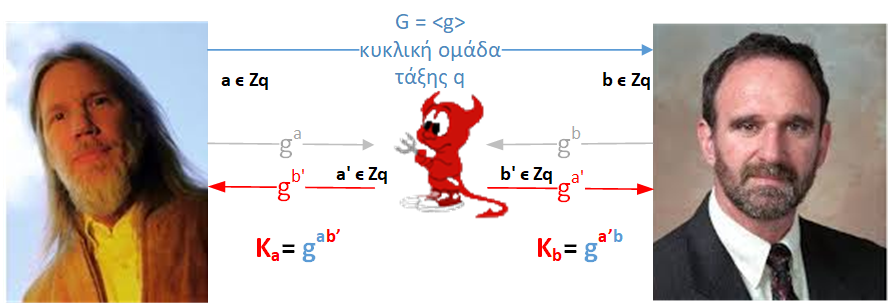
\includegraphics[scale=0.6]{dh-mitm.png}
\end{center} 
\pause 
Πώς είμαι σίγουρος ότι μιλάω με αυτόν που \emph{νομίζω} ότι μιλάω;
Λύση: ψηφιακές υπογραφές - ψηφιακό πιστοποιητικό (εγγύηση 'έμπιστου' τρίτου)
\end{frame}

\begin{frame}{Πραγματικά παραδείγματα}
\begin{block}{\href{https://www.schneier.com/blog/archives/2015/02/man-in-the-midd_7.html}{Superfish (02/2015)}}
	\begin{itemize}
		\item Προεγκατεστημένο λογισμικό Visual Discovery: προσπάθεια για εμφάνιση διαφημίσεων όχι με βάση κείμενο αλλά με βάση εικόνες \pause
		\item Παρακολούθηση δικτυακής κίνησης και μέσω https \pause
		\item Λογισμικό proxy που λειτουργεί ως MiTM \pause
		\item Εγκατάσταση και (self signed) ψηφιακού πιστοποιητικού \pause
	\end{itemize}
\end{block}
\pause
Και άλλες ανάλογες περιπτώσεις: πχ. \alert{\href{http://arstechnica.com/security/2015/11/dell-apologizes-for-https-certificate-fiasco-provides-removal-tool/}{DELL - 10/2015}}

\end{frame}


\section{Πηγές}
\begin{frame}{Βιβλιογραφία}
\begin{tiny}
\begin{itemize}
\item \href{ http://hdl.handle.net/11419/5439}{Παγουρτζής, Α., Ζάχος, Ε., ΓΠ, 2015. Υπολογιστική κρυπτογραφία. [ηλεκτρ. βιβλ.] Αθήνα:Σύνδεσμος Ελληνικών Ακαδημαϊκών Βιβλιοθηκών}
\item Jonathan Katz and Yehuda Lindell. Introduction to Modern Cryptography (Chapman and Hall/Crc Cryptography and Network Security Series). Chapman
and Hall/CRC, 2007
\item \href{http://goo.gl/b75I29}{Nigel Smart. Introduction to cryptography} 

\item Alptekin Kupcu. \href{https://goo.gl/l4GT2u}{Proofs In Cryptography}

\item S. Goldwasser and S. Micali. Probabilistic encryption. Journal of Computer and System Sciences, 28(2):270–299, 1984.
\item S. Micali, C. Rackoff, and B. Sloan. The notion of security for probabilistic cryptosystems. SIAM J. Computing, 17(2):412–426, 1988.

\item W. Diffie and M. Hellman. New directions in cryptography. IEEE Trans. Inf. Theor., 22(6):644-654, September 1976

\item Ivan Damgard, \href{http://goo.gl/mgAXC8}{A proof reading of some issues in cryptography}
\item Neil Koblitz, Alfred Menezes \href{https://goo.gl/GJNklR}{Another Look at “Provable Security”}

\item Dan Boneh (1998). "The Decision Diffie–Hellman Problem". ANTS-III: Proceedings of the Third International Symposium on Algorithmic Number Theory. Springer-Verlag: 48–63. doi:10.1007/bfb0054851

\item \href{https://www.schneier.com/}{Bruce Schneier's Blog}
\item \href{http://blog.cryptographyengineering.com/}{A Few Thoughts on Cryptographic Engineering}
\item \href{http://goo.gl/whmmb9}{Bristol Cryptography Blog}
 
\end{itemize}
\end{tiny}
\end{frame}

 
\end{document}
